%%%%%%%%%%%%%%%%%%%%%%%%%%%%%%%%%%%%%%%%%%%%%%%%%%%%%%%%%%%%%%%%%%%%%%%%%
\section{Network Choice Model}  %%%%%%%%%%%%%%%%%%%%%%%%%%%%%%%%%%%%%%%%%
\label{cr:sec:model}

Let $\mathcal{G} = (\mathcal{V}, \mathcal{E})$ be a directed graph on $N$ nodes (corresponding to items) and $M$ edges, with edge weights $w_{ij} > 0$ for all $(i, j) \in \mathcal{E}$.
We denote the out-neighborhood of node $i$ by $\mathcal{N}^+_i$ and its in-neighborhood by $\mathcal{N}^-_i$.
We consider the following choice process on $\mathcal{G}$.
A user starts at a node $i$ and is faced with alternatives $\mathcal{N}^+_i$.
The user chooses item $j$ and moves to the corresponding node.
At node $j$, the user is faced with alternatives $\mathcal{N}^+_j$ and chooses $k$, and so on.
At any time, the user can stop.
Figure~\ref{cr:fig:samplenet} gives an example of a graph and the alternatives available at a step of the process.

\begin{figure}
  \centering
  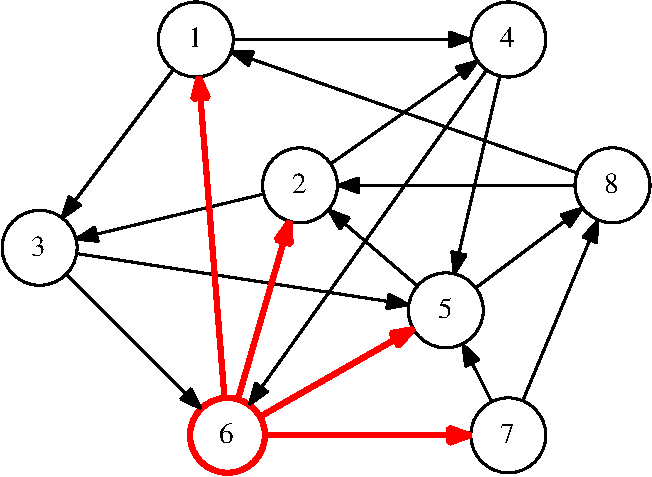
\includegraphics[scale=0.8]{cr-graph-example}
  \caption{An illustration of one step of the process.
  The user is at node 6 and can reach nodes $\mathcal{N}^+_6 = \{1, 2, 5, 7\}$.}
  \label{cr:fig:samplenet}
\end{figure}

To define the transition probabilities, we follow \citet{kumar2015inverting} and posit a probabilistic model of choice, which extends that of \citet{luce1959individual}.
For every node $i$ and every $j \in \mathcal{N}^+_i$, the probability that $j$ is selected among alternatives $\mathcal{N}^+_i$ can be written as
\begin{align}
\label{cr:eq:singlelik}
p_{ij} = \frac{w_{ij} \gamma_j}{\sum_{k \in \mathcal{N}^+_i} w_{ik} \gamma_k},
\end{align}
for some parameter vector $\bm{\gamma} = [\gamma_1 \ \cdots \ \gamma_N]^\Tr \in \mathbf{R}_{>0}^N$.
Intuitively, the parameter $\gamma_i$ can be interpreted as the utility of item $i$.
The edge weights are relevant in situations where the current context modulates the alternatives' utility;
for example, they can be used to encode the position or prominence of a link on a page in a hyperlink graph, or the distance between two locations in a mobility network.
Luce's original choice model is obtained by setting $w_{ij} \doteq \text{constant}$.
Note that $p_{ij}$ depends only on the out-neighborhood of node $i$.
As such, the choice process satisfies the Markov property, and we can think of the sequence of choices as a trajectory in a Markov chain.

In the context of this model, we can formulate the inference problem as follows.
Given a directed graph $\mathcal{G} = (\mathcal{V}, \mathcal{E})$, edge weights $\{ w_{ij} \}$ and data on the aggregate traffic at each node, find a parameter vector $\bm{\gamma}$ that fits the data.

\paragraph{Notation}
In some expressions, we use $\kappa$ to denote a constant that does not depend on the parameter vector $\bm{\gamma}$.
Its value can change from line to line.

%%%%%%%%%%%%%%%%%%%%%%%%%%%%%%%%%%%%%%%%%%%%%%%%%%%%%%%%%%%%%%%%%%%%%%%%%
\subsection{Sufficient Statistic}

We begin by showing that $\BigO{N}$ values summarizing the aggregate traffic at each node are a sufficient statistic of the transition counts.
Let $c_{ij}$ denote the number of transitions that occurred along edge $(i, j) \in \mathcal{E}$.
Starting from the transition probability defined in~\eqref{cr:eq:singlelik}, we can write the log-likelihood of $\bm{\gamma}$ given data $\mathcal{D} = \{ c_{ij} : (i, j) \in \mathcal{E} \}$ as
\begin{align}
\ell(\bm{\gamma} ; \mathcal{D})
    &= \sum_{(i,j) \in \mathcal{E}} c_{ij} \bigg[ \log w_{ij} \gamma_j - \log \sum_{k \in \mathcal{N}^+_i} w_{ik} \gamma_k \bigg] \nonumber \\
    &= \sum_{j = 1}^N \sum_{i \in \mathcal{N}^-_j}\!c_{ij} \log \gamma_j
       - \sum_{i = 1}^N \sum_{j \in \mathcal{N}^+_i}\!c_{ij} \log \sum_{k \in \mathcal{N}^+_i} w_{ik} \gamma_k
       + \sum_{(i,j) \in \mathcal{E}} c_{ij} \log w_{ij}, \nonumber \\
    &= \sum_{i = 1}^N \bigg[ c^-_i \log \gamma_i - c^+_i \log\!\sum_{k \in \mathcal{N}^+_i}\!w_{ik} \gamma_k \bigg] + \kappa, \label{cr:eq:loglik}
\end{align}
where $c^-_i = \sum_{j \in \mathcal{N}^-_i} c_{ji}$ and $c^+_i = \sum_{j \in \mathcal{N}^+_i} c_{ij}$ is the aggregate number of transitions arriving in and originating from $i$, respectively.
This formulation of the log-likelihood exhibits a key feature of the model:
the set of $2N$ counts $\{ (c^-_i, c^+_i) : i \in \mathcal{V} \}$ is a sufficient statistic of the $M = \BigO{N^2}$ counts $\{ c_{ij} : (i, j) \in \mathcal{E} \}$ for the parameters $\bm{\gamma}$.

\begin{theorem}
The set of aggregate transitions  $\{ (c^-_i, c^+_i) : i \in \mathcal{V} \}$ is a minimally sufficient statistic for the parameters $\bm{\gamma}$.
\end{theorem}

\begin{proof}
Let $f(\{ c_{ij} \} \mid \bm{\gamma})$ be the discrete probability density function of the data under the model with parameters $\bm{\gamma}$.
By Theorem $6.2.13$ in \citet{casella2002statistical}, $\{ (c^-_i, c^+_i) \}$ is a minimally sufficient statistic for $\bm{\gamma}$ if and only if, for any $\{ c_{ij} \}$ and $\{ d_{ij} \}$ in the support of $f$,
\begin{align}
\label{cr:eq:minsuff}
\begin{aligned}
\frac{ f(\{ c_{ij} \} \mid \bm{\gamma}) }{ f(\{ d_{ij} \} \mid \bm{\gamma}) }\ \text{is independent of $\bm{\gamma}$}
\iff (c^-_i, c^+_i) = (d^-_i, d^+_i) \quad \forall i.
\end{aligned}
\end{align}
Taking the log of the ratio on the left-hand side and using~\eqref{cr:eq:loglik}, we find that
\begin{align*}
\log \frac{ f(\{ c_{ij} \} \mid \bm{\gamma}) }{ f(\{ d_{ij} \} \mid \bm{\gamma}) } =
  \sum_{i = 1}^N \bigg[ (c^-_i\!-\!d^-_i) \log \gamma_i
                       - (c^+_i\!-\!d^+_i) \log\!\sum_{k \in \mathcal{N}^+_i}\!w_{ik} \gamma_k \bigg] + \kappa.
\end{align*}
From this, it is easy to see that the ratio of densities is independent of $\bm{\gamma}$ if and only if $c^-_i = d^-_i$ and $c^+_i = d^+_i$, which verifies~\eqref{cr:eq:minsuff}.
\end{proof}

In other words, it is enough to observe marginal information about the number of arrivals and departures at each node---we call this collective data the \emph{traffic} at a node---and no additional information can be gained by observing the full choice process.
This makes the model particularly attractive, because it means that it is unnecessary to track users across nodes.
In several applications of practical interest, tracking users is undesirable, difficult, or outright impossible, due to
\begin{enuminline}
\item privacy reasons,
\item monitoring costs, or
\item lack of data in existing datasets.
\end{enuminline}

Note that if we make the additional assumption that the flow in the network is conserved, then $c^-_i = c^+_i$.
If users' typical trajectories are made of many hops, it is reasonable to approximate $c^-_i$ or $c^+_i$ by using this assumption, should one of the two quantities be missing.

%%%%%%%%%%%%%%%%%%%%%%%%%%%%%%%%%%%%%%%%%%%%%%%%%%%%%%%%%%%%%%%%%%%%%%%%%
\subsection{Steady-State Inversion Problem}
% Also works if all the Markov trajectories are loops.

In recent work, \citet{kumar2015inverting} define the problem of \emph{steady-state inversion} as follows:
Given a strongly-connected directed graph $\mathcal{G} = (\mathcal{V}, \mathcal{E})$ with edge weights $\{ w_{ij} \}$ and a target distribution over the nodes $\bm{\pi}$, find the transition matrix of a Markov chain on $\mathcal{G}$ with stationary distribution $\bm{\pi}$.
As there are $M = \BigO{N^2}$ degrees of freedom (the transition probabilities) for $N$ constraints (the stationary distribution), the problem is in most cases underdetermined.
Following Luce's ideas, the transition probabilities are constrained to be proportional to a latent score of the destination node as per \eqref{cr:eq:singlelik}, thus reducing the number of parameters from $M$ to $N$.
Denote by $\bm{P}(\bm{s})$ the Markov-chain transition matrix parametrized with scores $\bm{s}$.
The score vector $\bm{s}$ is a solution for the steady-state inversion problem if and only if $\bm{\pi}^\Tr = \bm{\pi}^\Tr \bm{P}(\bm{s})$, or equivalently
\begin{align}
\label{cr:eq:balance}
\pi_i = \sum_{j \in \mathcal{N}^-_i} \frac{w_{ji} s_i}{\sum_{k \in \mathcal{N}^+_j} w_{jk} s_k} \pi_j \quad \forall i.
\end{align}
In order to formalize the connection between \citeauthor{kumar2015inverting}'s work and ours, we express the steady-state inversion problem as that of asymptotic maximum-likelihood estimation in the network choice model.
Suppose that we observe node-level traffic data $\mathcal{D} = \{ (c^-_i, c^+_i) : i \in \mathcal{V} \}$ about a trajectory of length $T$ starting at an arbitrary node.
We want to obtain an estimate of the parameters $\bm{\gamma}^\star$ by maximizing the average log-likelihood $\hat{\ell}(\bm{\gamma}) = \frac{1}{T} \ell (\bm{\gamma} ; \mathcal{D})$.
From standard convergence results for Markov chains \citep{kemeny1976finite}, it follows that as $\mathcal{G}$ is strongly connected, $\lim_{T \to \infty} c^-_i / T = \lim_{T \to \infty} c^+_i / T = \pi_i$.
Therefore,
\begin{align*}
\hat{\ell}(\bm{\gamma})
    = \sum_{i = 1}^N \bigg[ \frac{c^-_i}{T} \log \gamma_i - \frac{c^+_i}{T} \log \sum_{k \in \mathcal{N}^+_i} w_{ik} \gamma_k \bigg]
    \xrightarrow{T \to \infty} \sum_{i = 1}^N \pi_i \bigg[ \log \gamma_i - \log \sum_{k \in \mathcal{N}^+_i} w_{ik} \gamma_k \bigg].
\end{align*}
Let $\bm{\gamma}^\star$ be a maximizer of the average log-likelihood.
When $T \to \infty$, the optimality condition $\nabla \hat{\ell} = \bm{0}$ implies, for all $i$,
\begin{align}
&\frac{\partial \hat{\ell}(\bm{\gamma})}{\partial \gamma_i} \bigg|_{\bm{\gamma} = \bm{\gamma}^\star}
    = \frac{\pi_i}{\gamma^\star_i} - \sum_{j \in \mathcal{N}^-_i} \frac{w_{ji} \pi_j}{\sum_{k \in \mathcal{N}^+_j} w_{jk} \gamma^\star_k}
    = 0 \nonumber \\
&\qquad \iff \pi_i = \sum_{j \in \mathcal{N}^-_i} \frac{w_{ji} \gamma^\star_i}{\sum_{k \in \mathcal{N}^+_j} w_{jk} \gamma^\star_k} \pi_j. \label{cr:eq:optimality}
\end{align}
Comparing~\eqref{cr:eq:optimality} to~\eqref{cr:eq:balance}, it is clear that $\bm{\gamma}^\star$ is a solution of the steady-state inversion problem.
As such, the network choice model presented in this chapter can be viewed as a principled extension of the steady-state inversion problem to the finite-data case.


%%%%%%%%%%%%%%%%%%%%%%%%%%%%%%%%%%%%%%%%%%%%%%%%%%%%%%%%%%%%%%%%%%%%%%%%%
\subsection{MLE}
\label{cr:sec:maxlik}

The log-likelihood~\eqref{cr:eq:loglik} is not concave in $\bm{\gamma}$, but it can be made concave by using the standard reparametrization $\gamma_i = e^{\theta_i}$.
Therefore, any local minimum of the likelihood is a global minimum (c.f. Section~\ref{fi:sec:mle}).
Unfortunately, it turns out that the conditions guaranteeing that the ML estimate is well-defined (i.e., that it exists and is unique) are restrictive and impractical.

\begin{definition}[comparison graph]
Let $\mathcal{G} = (\mathcal{V}, \mathcal{E})$ be a directed graph and $\{ a_{ij} : (i,j) \in \mathcal{E} \}$ be non-negative numbers.
The \emph{comparison graph} induced by $\{ a_{ij} \}$ is the directed graph $\mathcal{G}' = (\mathcal{V}, \mathcal{E}')$, where $(i,j) \in \mathcal{E}'$ if and only if there is a node $k$ such that $i, j \in \mathcal{N}^+_k$ and $a_{kj} > 0$.
\end{definition}

The numbers $\{ a_{ij}\}$ in the definition can be loosely interpreted as transition counts (although they do not need to be integers).
Intuitively, there is an edge $(i, j)$ in the comparison graph whenever there is at least one instance in which $i$ and $j$ are among the alternatives and $j$ is selected.
The notion of comparison graph leads to a precise characterization of whether the ML estimate is well-defined or not, as shown by the next theorem---an extension of Theorem~\ref{fi:thm:mlboth} to the network choice model.

\begin{theorem}
\label{cr:thm:mlboth}
Let $\mathcal{G} = (\mathcal{V}, \mathcal{E})$ be a weighted, directed graph and $\{ (c^-_i, c^+_i) \}$ be the aggregate number of transitions arriving in and originating from $i$, respectively.
Let $\{ a_{ij} \}$ be any set of non-negative real numbers that satisfy
\begin{align*}
\sum_{j \in \mathcal{N}^-_i} a_{ji} = c^-_i, \quad
\sum_{j \in \mathcal{N}^+_i} a_{ij} = c^+_i \quad \forall i.
\end{align*}
Then, the maximizer of the log-likelihood~\eqref{cr:eq:loglik} exists and is unique (up to rescaling) if and only if the comparison graph induced by $\{ a_{ij} \}$ is strongly connected.
\end{theorem}

\begin{proof}
The proof borrows from \citet{hunter2004mm}, in particular from the proofs of Lemmas~$1$ and~$2$.
Using $\gamma_i = e^{\theta_i}$, we can rewrite the reparametrized log-likelihood using $\{ a_{ij} \}$ as
\begin{align*}
    \ell(\bm{\theta})
        = \sum_{i = 1}^N \sum_{j \in \mathcal{N}^+_i} a_{ij} \bigg[ \theta_j - \log \sum_{k \in \mathcal{N}^+_i} w_{ik} e^{\theta_k} \bigg],
\end{align*}
and, without loss of generality, we can assume that $\sum_i \theta_i = 0$ and $\min_{ij} w_{ij} = 1$.
We study the conditions under which
\begin{enuminline}
\item super-level sets of the likelihood function $\ell(\bm{\theta})$ are bounded, and
\item the likelihood function is strictly concave.
\end{enuminline}

First, we prove that the super-level set $\{ \bm{\theta} : \ell(\bm{\theta}) \ge c \}$ is bounded and compact for any $c$, if and only if the comparison graph is strongly connected.
The compactness of all super-level sets ensures that there is at least one maximizer.
Pick any unit-norm vector $\bm{u}$ such that $\sum_i u_i = 0$, and let $\bm{\theta} = s \bm{u}$
When $s \to \infty$, then $e^{\theta_i} > 0$ and $e^{\theta_j} \to 0 $ for some $i$ and $j$.
As the comparison graph is strongly connected, there is a path from $i$ to $j$, and along this path there must be two consecutive nodes $i', j'$ such that $e^{\theta_{i'}} > 0$ and $e^{\theta_{j'}} \to 0$.
The existence of the edge $(i',j')$ in the comparison graph means that there is a $k$ such that $i', j' \in \mathcal{N}^+_k$ and $a_{kj'} > 0$.
Therefore, the log-likelihood can be bounded as
\begin{align*}
\ell(\bm{\theta})
    \le a_{kj'} \bigg[ \theta_{j'} - \log \sum_{q \in \mathcal{N}^+_k} w_{kq} e^{\theta_q} \bigg]
    \le a_{kj'} \left[ \theta_{j'} - \log (e^{\theta_{j'}} + e^{\theta_{i'}}) \right],
\end{align*}
and $\lim_{s \to \infty} \ell(\bm{\theta}) = -\infty$.
Conversely, suppose that the comparison graph is not strongly connected and partition the vertices into two non-empty subsets $\mathcal{S}$ and $\mathcal{T}$ such that there is no edge from $\mathcal{S}$ to $\mathcal{T}$.
Let $c > 0$ be any positive constant, and take $\tilde{\theta}_i = \theta_i + c$ if $i \in \mathcal{S}$ and $\tilde{\theta}_i = \theta_i$ if $i \in \mathcal{T}$ (renormalize such that $\sum_i \tilde{\theta}_i = 0$).
Clearly, $\ell(\tilde{\bm{\theta}}) \ge \ell(\bm{\theta})$, and, by repeating this procedure, $\Norm{\bm{\theta}}$ can be driven to infinity without decreasing the likelihood.

Second, we prove that if the comparison graph is strongly connected, the log-likelihood is strictly concave (in $\bm{\theta}$).
In particular, for any $p \in (0,1)$,
\begin{align}
\label{cr:eq:strictconcav}
\ell \left[ p \bm{\theta} + (1-p) \bm{\eta} \right] \ge p \ell(\bm{\theta}) + (1-p) \ell(\bm{\eta}),
\end{align}
with equality if and only if $\bm{\theta} \equiv \bm{\eta}$ up to a constant shift.
Strict concavity ensures that there is at most one maximizer of log-likelihood.
We start with Hölder's inequality, which implies that, for positive $\{ x_k \}$ and $\{ y_k \}$, and $p \in (0,1)$,
\begin{align*}
\log \sum_k x_k^p y_k^{1-p} \le p \log \sum_k x_k + (1-p) \log \sum_k y_k.
\end{align*}
with equality if and only $x_k = c y_k$ for some $c > 0$.
Letting $x_k = w_{ik} e^{\theta_k}$ and $y_k = w_{ik} e^{\eta_k}$, we find that for all $i$
\begin{align}
\label{cr:eq:holderapp}
\begin{aligned}
\log \sum_{k \in \mathcal{N}^+_i} w_{ik} e^{p \theta_k + (1-p) \eta_k}
    \le p \log\!\sum_{k \in \mathcal{N}^+_i}\!w_{ik} e^{\theta_k} + (1-p) \log\!\sum_{k \in \mathcal{N}^+_i}\!w_{ik} e^{\eta_k},
\end{aligned}
\end{align}
with equality if and only if there exists $c \in \mathbf{R}$ such that $\theta_k = \eta_k + c$ for all $k \in \mathcal{N}^+_{i}$.
Multiplying by $a_{ij}$ and summing over $i$ and $j$ on both sides of~\eqref{cr:eq:holderapp} shows that the log-likelihood is concave in $\bm{\theta}$.
Now, consider any partition of the vertices into two non-empty subsets $\mathcal{S}$ and $\mathcal{T}$.
Because the comparison graph is strongly connected, there is always $k \in \mathcal{V}$, $i \in \mathcal{S}$ and $j \in \mathcal{T}$ such that $i, j \in \mathcal{N}^+_k$ and $a_{ki} > 0$.
Therefore, the left and right side of~\eqref{cr:eq:strictconcav} are equal if and only if $\bm{\theta} \equiv \bm{\eta}$ up to a constant shift.
\end{proof}

In order to verify the necessary and sufficient condition of Theorem~\ref{cr:thm:mlboth} given $\{ (c^-_i, c^+_i) \}$, we have to find a non-negative solution $\{ a_{ij} \}$ to the system of equations
\begin{align*}
\sum_{j \in \mathcal{N}^-_i} a_{ji} = c^-_i, \quad
\sum_{j \in \mathcal{N}^+_i} a_{ij} = c^+_i \quad \forall i.
\end{align*}
\citet{dines1926positive} presents a simple algorithm to find such a non-negative solution.
Alternatively, \citet{kumar2015inverting} suggest recasting the problem as one of maximum flow in a network.
However, the computational cost of running \citeauthor{dines1926positive}' or max-flow algorithms is significantly greater than that of running the inference algorithm that we develop later, in Section~\ref{cr:sec:algorithm}.

\paragraph{Example}
In order to illustrate Theorem~\ref{cr:thm:mlboth}, we describe an innocuous-looking example where the MLE does not exist.
Consider the network structure and traffic data depicted in Figure~\ref{cr:fig:badexample}.
The network is strongly connected and every node $i$ has positive incoming and outgoing traffic $c^-_i$ and $c^+_i$.
Nevertheless, the corresponding comparison graph is \emph{not} strongly connected, and it turns out that the likelihood can be made arbitrarily large by increasing $\gamma_1$, $\gamma_2$ and $\gamma_4$.
In this simple example, we indicate the edge transitions that generated the observed marginal traffic in bold.
Given this information, the comparison graph is easy to find, and the necessary and sufficient condition is easy to check.
But in general, finding a set of transitions that is compatible with given marginal per-node traffic data is a nontrivial computation.

\begin{figure}
  \begin{subfigure}{.49\textwidth}
    \centering
    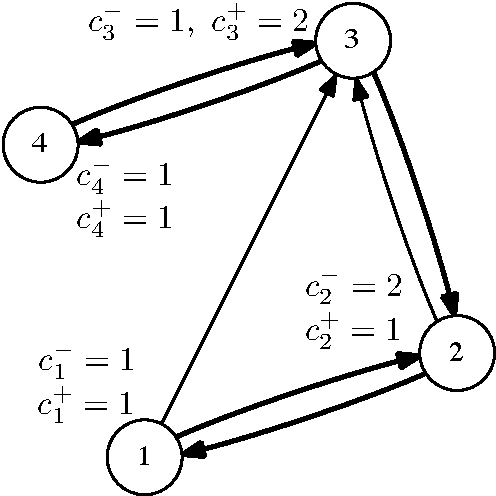
\includegraphics[width=.85\linewidth]{cr-ml-undefined}
    \caption{network structure}
  \end{subfigure}%
  \begin{subfigure}{.49\textwidth}
    \centering
    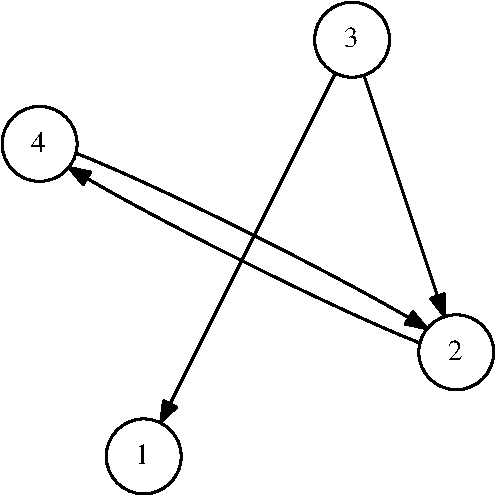
\includegraphics[width=.85\linewidth]{cr-ml-undefined-comp}
    \caption{comparison graph}
  \end{subfigure}
  \caption{An innocent-looking example where the ML estimate does not exist.
  The network structure, aggregate traffic data and compatible transitions are shown on the left.
  The comparison graph (right) is not strongly connected.}
  \label{cr:fig:badexample}
\end{figure}

\paragraph{Necessary Condition}
As the conditions of Theorem~\ref{cr:thm:mlboth} involve the observed traffic, we might ask the following question.
Is there a simpler condition on the structure of $\mathcal{G}$ such that the MLE is well-defined, given sufficiently many transitions?
We provide an answer in the form of a necessary condition for the uniqueness of the MLE that involves only the structure of the network.
We begin with a definition that uses the notion of \emph{hypergraph}, a generalized graph where edges can be any non-empty subset of nodes.

\begin{definition}[alternatives hypergraph]
Given a directed graph $\mathcal{G} = (\mathcal{V}, \mathcal{E})$, the \emph{alternatives hypergraph} is defined as $\mathcal{H} = (\mathcal{V}, \mathcal{A})$, with $\mathcal{A} = \{ \mathcal{N}^+_i : i \in \mathcal{V} \}$.
\end{definition}

Intuitively, $\mathcal{H}$ is the hypergraph induced by the sets of alternatives available at each node.
Equipped with this definition, we can state the following corollary of Theorem~\ref{cr:thm:mlboth}.

\begin{corollary}
\label{cr:thm:mlnecessary}
If the alternatives hypergraph is not connected, then for any data $\mathcal{D}$ there are $\bm{\gamma}$ and $\bm{\lambda}$ such that $\bm{\gamma} \neq c \bm{\lambda}$ for any $c \in \mathbf{R}_{>0}$ and $\ell(\bm{\gamma} ; \mathcal{D}) = \ell(\bm{\lambda} ; \mathcal{D}).$
\end{corollary}

\begin{proof}
If the alternatives hypergraph is disconnected, then for any data $\mathcal{D}$, the comparison graph is disconnected too.
Furthermore, the connected components of the comparison graph are subsets of those of the hypergraph.
Partition the vertices into two non-empty subsets $\mathcal{S}$ and $\mathcal{T}$ such that there is no hyperedge between $\mathcal{S}$ to $\mathcal{T}$ in the alternatives hypergraph.
Let $\mathcal{A} = \{ i : \mathcal{N}^+_i \subset \mathcal{S} \}$ and $\mathcal{B} = \{ i : \mathcal{N}^+_i \subset \mathcal{T} \}$.
By construction of the alternatives hypergraph, $\mathcal{A} \cap \mathcal{B} = \varnothing$ and $\mathcal{A} \cup \mathcal{B} = \mathcal{V}$.
The log-likelihood can be rewritten as
\begin{align*}
\ell(\bm{\theta}) =
    &\sum_{i \in \mathcal{A}} \sum_{j \in \mathcal{N}^+_i} a_{ij}
        \bigg[ \log \gamma_j - \log \sum_{k \in \mathcal{N}^+_i} w_{ik} \gamma_k \bigg] \\
    &+ \sum_{i \in \mathcal{B}} \sum_{j \in \mathcal{N}^+_i} a_{ij}
        \bigg[ \log \gamma_j - \log \sum_{k \in \mathcal{N}^+_i} w_{ik} \gamma_k \bigg].
\end{align*}
The sum over $\mathcal{A}$ involves only parameters related to nodes in $\mathcal{S}$, whereas the sum over $\mathcal{B}$ involves only parameters related to nodes in $\mathcal{T}$.
Because the likelihood is invariant to a rescaling of the parameters, it is easy to see that we can arbitrarily rescale the parameters of the vertices in either $\mathcal{S}$ or $\mathcal{T}$ without affecting the likelihood.
\end{proof}

The network of Figure~\ref{cr:fig:samplenet} illustrates an instance where even the necessary the condition fails:
although the graph $\mathcal{G}$ is strongly connected, its associated alternatives hypergraph $\mathcal{H}$ (depicted in Figure~\ref{cr:fig:samplehyp}) is disconnected, and no matter what the data $\mathcal{D}$ is, the ML estimate will never be uniquely defined.
Note that this problematic situation does not affect only carefully hand-crafted networks: the alternatives hypergraph of all three real-world networks considered in Section~\ref{cr:sec:experiments} are disconnected as well.

\begin{figure}
  \centering
  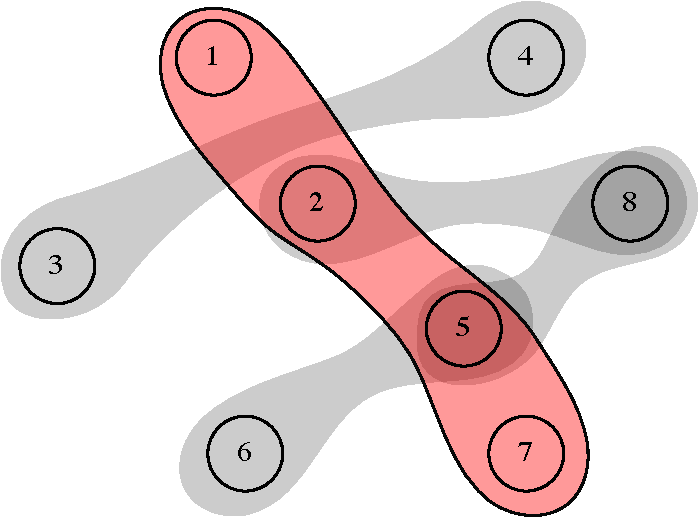
\includegraphics[width=.5\linewidth]{cr-graph-example-pref}
  \caption{The alternatives hypergraph associated with the network of Figure~\ref{cr:fig:samplenet}.
The hyperedge associated with $\mathcal{N}^+_6$ is highlighted in red.
Note that the component $\{3, 4\}$ is disconnected from the rest of the hypergraph.}
  \label{cr:fig:samplehyp}
\end{figure}
